\chapter{Multivariate models}\label{chap7}

\section{Solutions of Exercises}\label{sec71}
\begin{enumerate}[leftmargin=*]

	\item Show that $\mathbb{E}[u_1\text{PAER}]=\frac{\alpha_1}{1-\beta_1\alpha_1}\sigma^2_1$ assuming that $\mathbb{E}[u_1u_2]=0$ where $Var(u_1)=\sigma^2_1$ in the effect of institutions on per capita GDP.
	
	\textbf{Answer}
	
	The point of departure is the following \textit{simultaneous structural} economic model:
	\begin{align}\label{eq:str1}
		\log(\text{pcGDP95}_i)=\beta_1+\beta_2\text{PAER}_i+\beta_3 \text{Africa}+\beta_4 \text{Asia}+\beta_5 \text{Other}+u_{1i},
	\end{align}
	\begin{align}\label{eq:str2}
		\text{PAER}_i=\alpha_1+\alpha_2\log(\text{pcGDP95}_i)+\alpha_3\log(\text{Mort}_i)+u_{2i},
	\end{align}

where \textit{pcGDP95}, \textit{PAER} and \textit{Mort} are the per capita gross domestic product (GDP) in 1995, the average index of protection against expropriation between 1985 and 1995, and the settler mortality rate during the time of colonization. \textit{Africa}, \textit{Asia} and \textit{Other} are dummies for continents, with \textit{America} as the baseline group.

Replacing Equation \ref{eq:str2} into Equation \ref{eq:str1}, and solving for $\log(\textit{pcGDP95})$,
\begin{align}\label{eq:red1}
	\log(\text{pcGDP95}_i)=\pi_1+\pi_2\log(\text{Mort}_i)+\pi_3 \text{Africa}+\pi_4 \text{Asia}+\pi_5 \text{Other}+e_{1i},   
\end{align}

where $\pi_1=\frac{\beta_1+\beta_2\alpha_1}{1-\beta_2\alpha_2}$, $\pi_2=\frac{\beta_2\alpha_3}{1-\beta_2\alpha_2}$, $\pi_3=\frac{\beta_3}{1-\beta_2\alpha_2}$, $\pi_4=\frac{\beta_4}{1-\beta_2\alpha_2}$, 
$\pi_5=\frac{\beta_5}{1-\beta_2\alpha_2}$, and $e_1=\frac{\beta_2u_2+u_1}{1-\beta_2\alpha_2}$.

Then, replacing Equation \ref{eq:red1} into Equation \ref{eq:str2}, and solving for \textit{PAER},
\begin{align}\label{eq:red2}
	\text{PAER}_i=\gamma_1+\gamma_2\log(\text{Mort}_i)+\gamma_3 \text{Africa}+\gamma_4 \text{Asia}+\gamma_5 \text{Other}+e_{2i},
\end{align}
where $\gamma_1=\frac{\alpha_1+\alpha_2\beta_1}{1-\beta_2\alpha_2}$, $\gamma_2=\frac{\alpha_3}{1-\beta_2\alpha_2}$, $\gamma_3=\frac{\alpha_2\beta_3}{1-\beta_2\alpha_2}$, $\gamma_4=\frac{\alpha_2\beta_4}{1-\beta_2\alpha_2}$,
$\gamma_5=\frac{\alpha_2\beta_5}{1-\beta_2\alpha_2}$, and $e_2=\frac{\alpha_2u_1+u_2}{1-\beta_2\alpha_2}$.

Then, $\mathbb{E}[u_1\text{PAER}]=\mathbb{E}\left[u_1(\gamma_1+\gamma_2\log(\text{Mort}_i)+\gamma_3 \text{Africa}+\gamma_4 \text{Asia}+\gamma_5 \text{Other}+e_{2i})\right]=\mathbb{E}\left[u_1\left(\frac{\alpha_2u_1+u_2}{1-\beta_2\alpha_2}\right)\right]=\frac{\alpha_2}{1-\beta_2\alpha_2}\sigma^2_1$ given the assumptions.      

\item Show that $\beta_2=\pi_2/\gamma_2$ in the effect of institutions on per capita GDP.

\textbf{Answer}

Given that $\pi_2=\frac{\beta_2\alpha_3}{1-\beta_2\alpha_2}$ and $\gamma_2=\frac{\alpha_3}{1-\beta_2\alpha_2}$ from the previous exercise, consequently, $\beta_2=\pi_2/\gamma_2$.

\item \textbf{The effect of institutions on per capita gross domestic product continues}

Use the \textit{rmultireg} command from the \textit{bayesm} package to perform inference in the example of the effect of institutions on per capita GDP.

\textbf{Answer}

\begin{tcolorbox}[enhanced,width=4.67in,center upper,
	fontupper=\large\bfseries,drop shadow southwest,sharp corners]
	\textit{R code. The effect of institutions on per capita GDP}
	\begin{VF}
		\begin{lstlisting}[language=R]
rm(list = ls())
set.seed(010101)
DataInst <- read.csv("https://raw.githubusercontent.com/besmarter/BSTApp/refs/heads/master/DataApp/4Institutions.csv", sep = ",", header = TRUE, quote = "")
attach(DataInst)
Y <- cbind(logpcGDP95, PAER)
X <- cbind(1, logMort, Africa, Asia, Other)
M <- dim(Y)[2]
K <- dim(X)[2]
# Hyperparameters
B0 <- matrix(0, K, M)
c0 <- 100
V0 <- c0*diag(K)
Psi0 <- 5*diag(M)
a0 <- 5
S <- 10000 #Number of posterior draws
betadraw = matrix(double(S*K*M), ncol=K*M)
Sigmadraw = matrix(double(S*M*M), ncol=M*M)
pb <- winProgressBar(title = "progress bar", min = 0, max = S, width = 300)
for (s in 1:S) {
	Results <- bayesm::rmultireg(Y, X, Bbar = B0, A = solve(V0), nu = a0, V = Psi0)
	betadraw[s,] <- Results$B
	Sigmadraw[s,] <- Results$Sigma
	setWinProgressBar(pb, s, title=paste( round(s/S*100, 0), "% done"))
}
close(pb)
summary(coda::mcmc(betadraw))
summary(coda::mcmc(Sigmadraw))
\end{lstlisting}
	\end{VF}
\end{tcolorbox} 
 
	\item \textbf{Demand and supply simulation}

Given the structural demand-supply model:
\begin{align*}
	q_i^d&=\beta_1+\beta_2p_i+\beta_3y_i+\beta_4pc_i+\beta_5ps_i+u_{i1}\\
	q_i^s&=\alpha_1+\alpha_2p_i+\alpha_3er_i+u_{i2},
\end{align*}
where $q^d$ is demand, $q^s$ is supply, $p$, $y$, $pc$, $ps$ and $er$ are price, income, complementary price, substitute price, and exchange rate. Complementary and substitute prices are prices of a complementary and substitute goods of $q$. Assume that $\bm{\beta}=\left[5 \ -0.5 \ 0.8 \ -0.4 \ 0.7\right]^{\top}$, $\bm{\alpha}=\left[-2 \ 0.5 \ -0.4\right]^{\top}$, $u_1\sim N(0, 0.5^2)$ and $u_2\sim N(0, 0.5^2)$. In addition, assume that $y\sim N(10,1)$, $pc\sim N(5,1)$, $ps\sim N(5,1)$ and $tc\sim N(15,1)$.
\begin{itemize}
	\item Find the \textit{reduce-form} model using that in equilibrium demand and supply are equal, that is, $q^d=q^s$. This condition defines the observable quantity ($q$).
	\item Simulate $p$ and $q$ from the \textit{reduce-form} equations.
	\item Preform inference of the \textit{reduce-form} model using the \textit{rmultireg} command from the \textit{bayesm} package.
	\item Use the posterior draws of the \textit{reduce-form} parameters to perform inference of the \textit{structural} parameters. Any issue? Hint: Are all \textit{structural} parameters exactly identified?   
\end{itemize}

\textbf{Answer}

We should equal demand and supply, and solve for price,
\begin{align*}
	p=\pi_1+\pi_2 er + \pi_3 y + \pi_4 pc + \pi_5 ps + v_1,
\end{align*}
where $\pi_1=\frac{\alpha_1-\beta_1}{\beta_2-\alpha_2}$, $\pi_2=\frac{\alpha_3}{\beta_2-\alpha_2}$, $\pi_3=\frac{-\beta_3}{\beta_2-\alpha_2}$, $\pi_4=\frac{-\beta_4}{\beta_2-\alpha_2}$, $\pi_5=\frac{-\beta_5}{\beta_2-\alpha_2}$, and $v_1=\frac{u_2-u_1}{\beta_2-\alpha_2}$ given $\beta_2\neq\alpha_2$, that is, the equations should be independent. This condition is given by economic theory due to $\beta_2<0$ and $\alpha_2>0$, the effect of price on demand and supply should be negative and positive, respectively.

The equation of price into the demand equation gives
\begin{align*}
	q=\tau_1+\tau_2 er + \tau_3 y + \tau_4 pc + \tau_5 ps + v_2,
\end{align*}

where $\tau_1=\beta_1+\beta_2\pi_1$, $\tau_2=\beta_2\pi_2$, $\tau_3=\beta_2\pi_3+\beta_3$, $\tau_4=\beta_2\pi_4+\beta_4$, $\tau_5=\beta_2\pi_5+\beta_5$, and $v_2=\beta_2v_1+u_1$. We can use the equations para $\pi_k$ and $\tau_k$, $k=\left\{1,2,3,4,5\right\}$ to simulate the \textit{reduced-form} equations.

Observe that estimating the \textit{reduced-form} equations, we can get the \textit{structural} parameters for the demand equation, $\beta_2=\tau_2/\pi_2$ ($\pi_2\neq 0$), $\beta_3=\tau_3-\beta_2\pi_3$, $\beta_4=\tau_4-\beta_2\pi_4$ and $\beta_5=\tau_5-\beta_2\pi_5$, whereas the \textit{structural} parameters of the supply equation cannot be recovered just in one way, $\alpha_2=\beta_2+\beta_3/\pi_3=\beta_2+\beta_4/\pi_4=\beta_2+\beta_5/\pi_5$. This in turn implies different values for  $\alpha_3=\pi_2(\beta_2-\alpha_2)$. This is because the demand equation is \textit{exactly identified}, whereas the supply equation is \textit{over identified}. 

In this exercise, $K=5$, $M=2$, $K_1=4$, $K_2=2$, $M_1=2$ and $M_2=2$. This means that $K-K_1=1=M-1$ and $K-K_2=3>M-1=1$, that is, the order condition says that both equations (demand and supply) satisfy the necessary condition of identification, the demand would be \textit{exactly identified}, and the supply equation would be \textit{over identified}.

Regarding the rank condition (necessary and sufficient), let's see the identification matrix:
\begin{table}[!h]
	%\noautomaticrules
	\tabletitle{Identification matrix.}\label{tab:71}%
	\begin{tabular}{ccccccc}
		q    & p & constant & er & y & pc & ps \\
		\hline
		1 & -$\beta_2$ & -$\beta_1$ & 0 & -$\beta_3$ & -$\beta_4$ & -$\beta_5$\\
		1 & -$\alpha_2$ & $-\alpha_1$ & -$\alpha_3$ & 0 & 0 & 0 \\
	\end{tabular}
\end{table}

The demand equation excludes the exchange rate (\textit{exclusion restriction}), and given $\alpha_3\neq 0$, that is, the exchange rate is relevant in the supply equation, then the rank condition is satisfied in the demand equation. The supply equation excludes the income, the complementary price and substitute price (\textit{exclusion restrictions}), then as far as $\beta_k\neq 0$ for any $k=\left\{3,4,5\right\}$, the rank condition is satisfied in the supply equation.

The following code shows how to do the simulation, and perform inference in this exercise. We can see that all 95\% credible intervals encompass the population parameters, and the posterior means are very close to them.
 
\begin{tcolorbox}[enhanced,width=4.67in,center upper,
	fontupper=\large\bfseries,drop shadow southwest,sharp corners]
	\textit{R code. Demand and supply simulation}
	\begin{VF}
		\begin{lstlisting}[language=R]
rm(list = ls()); set.seed(12345)
B0 <- 5; B1 <- -0.5; B2 <- 0.8; B3 <- -0.4; B4 <- 0.7; SD <- 0.5
A0 <- -2; A1 <- 0.5; A2 <- -0.4; SS <- 0.5
P0 <- (A0-B0)/(B1-A1); P2 <- -B2/(B1-A1); P3 <- -B3/(B1-A1); P1 <- A2/(B1-A1); P4 <- -B4/(B1-A1)
T0 <- B0+B1*P0; T2 <- B2+B1*P2; T3 <- B3+B1*P3; T1 <- B1*P1; T4 <- B4+B1*P4;
n <- 5000
ED <- rnorm(n, 0, SD); ES <- rnorm(n, 0, SS)
VP <- (ES-ED)/(B1-A1); UQ <- B1*VP+ED
y <- rnorm(n, 10, 1); pc <- rnorm(n, 5, 1); er <- rnorm(n, 15, 1); ps <- rnorm(n, 5, 1);
p <- P0+P1*er+P2*y+P3*pc+P4*ps+VP
q <- T0+T1*er+T2*y+T3*pc+T4*ps+UQ
#Inference
Y <- cbind(p, q); X <- cbind(1, er, y, pc, ps)
M <- dim(Y)[2]; K <- dim(X)[2]
# Hyperparameters
B0 <- matrix(0, K, M); c0 <- 100; V0 <- c0*diag(K)
Psi0 <- 5*diag(M); a0 <- 5; S <- 10000 #Posterior draws
betadraw = matrix(double(S*K*M), ncol=K*M)
Sigmadraw = matrix(double(S*M*M), ncol=M*M)
pb <- winProgressBar(title = "progress bar", min = 0, max = S, width = 300)
for (s in 1:S) {
	Results <- bayesm::rmultireg(Y, X, Bbar = B0, A = solve(V0), nu = a0, V = Psi0)
	betadraw[s,] <- Results$B
	Sigmadraw[s,] <- Results$Sigma
	setWinProgressBar(pb, s, title=paste( round(s/S*100, 0), "% done"))
}
close(pb)
summary(coda::mcmc(betadraw))
summary(coda::mcmc(Sigmadraw))
beta2 <- betadraw[,7]/betadraw[,2] # Effect of price on demand 
summary(coda::mcmc(beta2))
beta3 <- betadraw[,8] - beta2*betadraw[,3] # Effect of income on demand
summary(coda::mcmc(beta3))
beta4 <- betadraw[,9] - beta2*betadraw[,4] # Effect of complementary price on demand
summary(coda::mcmc(beta4))
beta5 <- betadraw[,10] - beta2*betadraw[,5] # Effect of substitute price  on demand
summary(coda::mcmc(beta5))
\end{lstlisting}
	\end{VF}
\end{tcolorbox}

\item \textbf{Utility demand continues}

\begin{itemize}
	\item Run the \textbf{Utility demand} application using our GUI and the information in the dataset \textit{Utilities.csv}. Hint: This file should be modified to agree the structure that requires our GUI (see the dataset \textit{5Institutions.csv} in the folder \textit{DataApp} of our GitHub repository -\textbf{https://github.com/besmarter/BSTApp}- for a template).
	\item Program from scratch the Gibbs sampler algorithm in this application.   
\end{itemize}

\textbf{Answer}

\begin{tcolorbox}[enhanced,width=4.67in,center upper,
	fontupper=\large\bfseries,drop shadow southwest,sharp corners]
	\textit{R code. Utility demand in Colombia, Gibss sampler}
	\begin{VF}
		\begin{lstlisting}[language=R]
rm(list = ls()); set.seed(010101); library(dplyr)
DataUt <- read.csv("https://raw.githubusercontent.com/besmarter/BSTApp/refs/heads/master/DataApp/Utilities.csv", sep = ",", header = TRUE, quote = "")
DataUtEst <- DataUt %>% filter(Electricity != 0 & Water !=0 & Gas != 0)
attach(DataUtEst)
y1 <- log(Electricity); y2 <- log(Water); y3 <- log(Gas)
X1 <- cbind(1, LnPriceElect, LnPriceWater, LnPriceGas, IndSocio1, IndSocio2, Altitude, Nrooms, HouseholdMem, Lnincome)
X2 <- cbind(1, LnPriceElect, LnPriceWater, LnPriceGas, IndSocio1, IndSocio2, Nrooms, HouseholdMem)
X3 <- cbind(1, LnPriceElect, LnPriceWater, LnPriceGas, IndSocio1, IndSocio2, Altitude, Nrooms, HouseholdMem)
y <- c(y1, y2, y3)
X <- as.matrix(Matrix::bdiag(X1, X2, X3))
M <- 3; K1 <- dim(X1)[2]; K2 <- dim(X2)[2]; K3 <- dim(X3)[2] 
K <- K1 + K2 + K3; N <- length(y1)
# Hyperparameters
b0 <- rep(0, K); c0 <- 100; B0 <- c0*diag(K)
B0i <- solve(B0); Psi0 <- 5*diag(M); Psi0i <- solve(Psi0)
a0 <- M; IN <- diag(N); an <- a0 + N
#Posterior draws
S <- 6000; burnin <- 1000; thin <- 1
tot <- S+burnin
# Gibbs functions
PostBeta <- function(Sigma){
	Aux <- solve(Sigma)%x%IN
	Bn <- solve(B0i + t(X)%*%Aux%*%X)
	bn <- Bn%*%(B0i%*%b0 + t(X)%*%Aux%*%y)
	Beta <- MASS::mvrnorm(1, bn, Bn)
	return(Beta)
}
PostSigma <- function(Beta){
	B1 <- Beta[1:K1]; B2 <- Beta[(K1+1):(K1+K2)]; B3 <- Beta[(K1+K2+1):(K1+K2+K3)]
	U1 <- y1 - X1%*%B1; U2 <- y2 - X2%*%B2; U3 <- y3 - X3%*%B3
	U <- cbind(U1, U2, U3)
	Psin <- solve(Psi0i + t(U)%*%U)
	Sigmai <- rWishart::rWishart(1, df = an, Sigma = Psin)
	Sigma <- solve(Sigmai[,,1]) 
	return(Sigma)
}
PostBetas <- matrix(0, tot, K)
PostSigmas <- matrix(0, tot, M*(M+1)/2); Beta <- rep(1, K)
pb <- winProgressBar(title = "progress bar", min = 0, max = tot, width = 300)
for(s in 1:tot){
	Sigma <- PostSigma(Beta = Beta); PostSigmas[s,] <- matrixcalc::vech(Sigma)
	Beta <- PostBeta(Sigma = Sigma); 	PostBetas[s,] <- Beta
	setWinProgressBar(pb, s, title=paste( round(s/tot*100, 0),"% done"))
}
close(pb)
keep <- seq((burnin+1), tot, thin)
Bs <- PostBetas[keep,]; summary(coda::mcmc(Bs))
Sigmas <- PostSigmas[keep,]; summary(coda::mcmc(Sigmas))
\end{lstlisting}
	\end{VF}
\end{tcolorbox} 

\begin{tcolorbox}[enhanced,width=4.67in,center upper,
	fontupper=\large\bfseries,drop shadow southwest,sharp corners]
	\textit{R code. Utility demand in Colombia, results}
	\begin{VF}
		\begin{lstlisting}[language=R]
keep <- seq((burnin+1), tot, thin)
Bs <- PostBetas[keep,]; summary(coda::mcmc(Bs))
Sigmas <- PostSigmas[keep,]; summary(coda::mcmc(Sigmas))
Quantiles for each variable:
						2.5%      25%       50%      75%    97.5%
Const         0.43304  1.04508  1.337751  1.64728  2.25228
LnPriceElect -2.40343 -2.05533 -1.882159 -1.70463 -1.35979
LnPriceWater -0.44027 -0.38524 -0.356049 -0.32676 -0.27021
LnPriceGas   -0.21665 -0.13807 -0.098877 -0.05712  0.01673
IndSocio1    -0.87408 -0.78454 -0.736561 -0.68898 -0.59137
IndSocio2    -0.24504 -0.18344 -0.150827 -0.11845 -0.06029
Altitude     -0.27153 -0.23866 -0.221539 -0.20468 -0.17325
Nrooms        0.04598  0.06191  0.069971  0.07837  0.09379
HouseholdMem  0.06610  0.07999  0.087320  0.09406  0.10708
Lnincome      0.03897  0.05516  0.063130  0.07152  0.08751
Const         0.88247  1.73546  2.162290  2.60793  3.48450
LnPriceElect -0.83128 -0.31258 -0.051838  0.20446  0.72087
LnPriceWater -0.49760 -0.40946 -0.363138 -0.31943 -0.23498
LnPriceGas    0.05880  0.16932  0.228734  0.28677  0.39226
IndSocio1    -0.63928 -0.50417 -0.427978 -0.35529 -0.21024
IndSocio2    -0.50363 -0.40976 -0.359576 -0.30929 -0.21097
Nrooms        0.05733  0.08126  0.093291  0.10550  0.12935
HouseholdMem  0.09984  0.12098  0.132126  0.14265  0.16290
Const        -2.26403 -1.57842 -1.201124 -0.84494 -0.15985
LnPriceElect -2.41128 -2.00330 -1.786150 -1.57292 -1.17185
LnPriceWater -0.10791 -0.03978 -0.003399  0.03329  0.10082
LnPriceGas   -0.76450 -0.67575 -0.627062 -0.57949 -0.48807
IndSocio1    -0.91346 -0.80094 -0.743421 -0.68334 -0.57228
IndSocio2    -0.31613 -0.24086 -0.202828 -0.16367 -0.08824
Altitude      0.24986  0.28987  0.310784  0.33183  0.37126
Nrooms        0.06071  0.07899  0.089606  0.09949  0.11842
HouseholdMem  0.14485  0.16148  0.169509  0.17797  0.19467
Sigmas <- PostSigmas[keep,]
summary(coda::mcmc(Sigmas))
        2.5%     25%     50%     75%   97.5%
var1 0.19664 0.20567 0.21072 0.21593 0.22636
var2 0.08201 0.09289 0.09865 0.10447 0.11623
var3 0.05222 0.06015 0.06452 0.06903 0.07799
var4 0.47390 0.49575 0.50789 0.52046 0.54446
var5 0.07355 0.08672 0.09381 0.10061 0.11427
var6 0.29259 0.30618 0.31384 0.32140 0.33700
\end{lstlisting}
	\end{VF}
\end{tcolorbox} 


\item \textbf{Simulation exercise of instrumental variables continues}

\begin{enumerate}
	\item Use the setting of the simulation exercise of instrumental variables to analyze what happens when the instrument is weak, for instance, setting $\gamma_2=0.2$, and compare the performance of the posterior means of the ordinary and instrumental models.
	\item Perform a simulation that helps to analyze how the degree of exogeneity of the instrument affects the performance of the posterior mean of the instrumental variable model.	 
\end{enumerate}

\textbf{Answer}

\begin{tcolorbox}[enhanced,width=4.67in,center upper,
	fontupper=\large\bfseries,drop shadow southwest,sharp corners]
	\textit{R code. Simulation exercise, sampling properties of instrumental variable}
	\begin{VF}
		\begin{lstlisting}[language=R]
rm(list = ls())
set.seed(010101)
N <- 100
k <- 2
B <- rep(1, k)
G <- c(1, 0.2)
s12 <- 0.8
SIGMA <- matrix(c(1, s12, s12, 1), 2, 2)
z <- rnorm(N); # w <- rnorm(N)
Z <- cbind(1, z); w <- matrix(1,N,1)
S <- 100
U <- replicate(S, MASS::mvrnorm(n = N, mu = rep(0, 2), SIGMA))
x <- G[1] + G[2]*z + U[,2,]
y <- B[1] + B[2]*x + U[,1,]
VarX <- G[2]^2+1 # Population variance of x
EU1U2 <- s12 # Covariance U1
BiasPopB2 <- EU1U2/VarX
# Hyperparameters
d0 <- 0.001/2
a0 <- 0.001/2
b0 <- rep(0, k)
c0 <- 1000
B0 <- c0*diag(k)
B0i <- solve(B0)
g0 <- rep(0, 2)
G0 <- 1000*diag(2)
G0i <- solve(G0)
nu <- 3
Psi0 <- nu*diag(2)
# MCMC parameters
mcmc <- 5000
burnin <- 1000
tot <- mcmc + burnin
thin <- 1
# Gibbs sampling
Gibbs <- function(x, y){
	Data <- list(y = y, x = x, w = w, z = Z)
	Mcmc <- list(R = mcmc, keep = thin, nprint = 0)
	Prior <- list(md = g0, Ad = G0i, mbg = b0, Abg = B0i, nu = nu, V = Psi0)
	RestIV <- bayesm::rivGibbs(Data = Data, Mcmc = Mcmc, Prior = Prior)
	PostBIV <- mean(RestIV[["betadraw"]])
	ResLM <- MCMCpack::MCMCregress(y ~ x + w - 1, b0 = b0, B0 = B0i, c0 = a0, d0 = d0)
	PostB <- mean(ResLM[,1])
	Res <- c(PostB,PostBIV)
	return(Res)
}
PosteriorMeans <- sapply(1:S, function(s) {Gibbs(x = x[,s], y = y[,s])})
rowMeans(PosteriorMeans)
1.781513 1.470648
\end{lstlisting}
	\end{VF}
\end{tcolorbox} 

Figure \ref{fig71} shows that having a \textit{weak instrument} generates poor performance of the posterior means of the variable instrumental model. Observe that the mean of the posterior means is less precise and biased. This is due to an identification problem in the likelihood function of $y$ and $x_s$ given $z$ (see \cite[Chap.~7]{rossi2005bayesian}).

\begin{figure}
	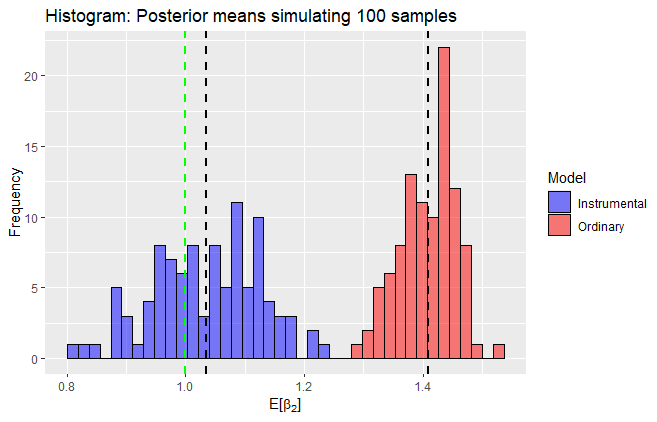
\includegraphics[width=340pt, height=200pt]{Chapters/chapter7/figures/Fig71.png}
	\caption[List of figure caption goes here]{Histogram of posterior means to assess the effects of \textit{weakness} of the instrument: Ordinary and instrumental models.}\label{fig71}
\end{figure}


\begin{tcolorbox}[enhanced,width=4.67in,center upper,
	fontupper=\large\bfseries,drop shadow southwest,sharp corners]
	\textit{R code. Simulation exercise, sampling properties of instrumental variable}
	\begin{VF}
		\begin{lstlisting}[language=R]
# Endogenous instruments
rm(list = ls())
set.seed(010101)
N <- 100
k <- 2
B <- rep(1, k)
G <- c(1, 1)
delta <- 0.2 # Effect of instrument on y
s12 <- 0.8
SIGMA <- matrix(c(1, s12, s12, 1), 2, 2)
z <- rnorm(N); # w <- rnorm(N)
Z <- cbind(1, z); w <- matrix(1,N,1)
S <- 100
U <- replicate(S, MASS::mvrnorm(n = N, mu = rep(0, 2), SIGMA))
x <- G[1] + G[2]*z + U[,2,]
y <- B[1] + B[2]*x + delta*z + U[,1,]
VarX <- G[2]^2+1 # Population variance of x
EU1U2 <- s12 # Covariance U1
BiasPopB2 <- EU1U2/VarX
# Hyperparameters
d0 <- 0.001/2
a0 <- 0.001/2
b0 <- rep(0, k)
c0 <- 1000
B0 <- c0*diag(k)
B0i <- solve(B0)
g0 <- rep(0, 2)
G0 <- 1000*diag(2)
G0i <- solve(G0)
nu <- 3
Psi0 <- nu*diag(2)
# MCMC parameters
mcmc <- 5000
burnin <- 1000
tot <- mcmc + burnin
thin <- 1
# Gibbs sampling
Gibbs <- function(x, y){
	Data <- list(y = y, x = x, w = w, z = Z)
	Mcmc <- list(R = mcmc, keep = thin, nprint = 0)
	Prior <- list(md = g0, Ad = G0i, mbg = b0, Abg = B0i, nu = nu, V = Psi0)
	RestIV <- bayesm::rivGibbs(Data = Data, Mcmc = Mcmc, Prior = Prior)
	PostBIV <- mean(RestIV[["betadraw"]])
	ResLM <- MCMCpack::MCMCregress(y ~ x + w - 1, b0 = b0, B0 = B0i, c0 = a0, d0 = d0)
	PostB <- mean(ResLM[,1])
	Res <- c(PostB,PostBIV)
	return(Res)
}
PosteriorMeans <- sapply(1:S, function(s) {Gibbs(x = x[,s], y = y[,s])})
rowMeans(PosteriorMeans)
1.508009 1.217419
\end{lstlisting}
	\end{VF}
\end{tcolorbox} 

A simple way to assess the effects of \textit{endogeneity} of the instrument in the instrumental variable model is to introduce the instrument into the \textit{structural equation}, but assume that $\mathbb{E}[yz|x_s]=0$. In particular, we generate $y_i=\beta_1+\beta_2 x_{si} + \beta_3 z_i + \mu_i$, but estimate $y_i=\beta_1+\beta_2 x_{si} + \mu_i$. Figure \ref{fig72} shows that assuming that an instrument is exogenous, when actually it is not, generates bias in the posterior mean of the instrumental variable model. Observe that \textit{exogeneity} of the instrument is equivalent to the dogmatic prior belief that the instrument does not affect the structural equation. Thus, \cite{Conley2012} propose to assess the plausibility of the \textit{exclusion restrictions} ($\beta_3=0$ and $\gamma_2\neq 0$) defining \textit{plausible exogeneity} as having prior information that the effect of the instrument in the \textit{structural equation} is near zero, but perhaps not exactly zero.  

\begin{figure}
	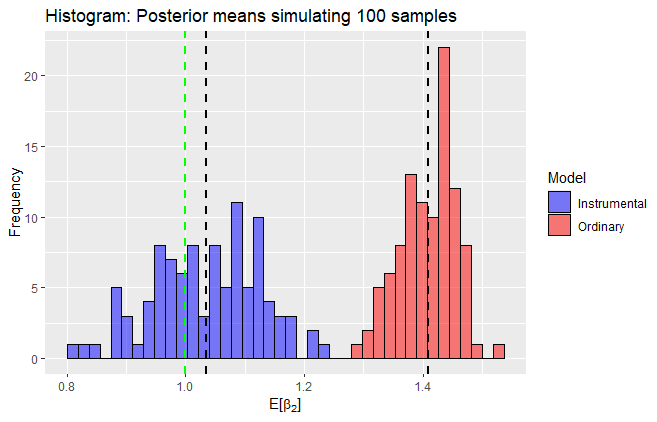
\includegraphics[width=340pt, height=200pt]{Chapters/chapter7/figures/Fig71.png}
	\caption[List of figure caption goes here]{Histogram of posterior means to assess the effects of \textit{endogeneity} of the instrument: Ordinary and instrumental models.}\label{fig72}
\end{figure}

\item \textbf{Simulation exercise of instrumental variables continues II}

Program from scratch the Gibbs sampling algorithm of the instrumental model for the simulation exercise of the instrumental variables.

\textbf{Answer}

The following code shows how to implement the Gibbs sampling algorithm from scratch. We observe that all posterior means are close to the population values, and 95\% credible intervals encompass them.

\begin{tcolorbox}[enhanced,width=4.67in,center upper,
	fontupper=\large\bfseries,drop shadow southwest,sharp corners]
	\textit{R code. Simulation exercise, Gibss sampling instrumental model}
	\begin{VF}
		\begin{lstlisting}[language=R]
rm(list = ls()); set.seed(010101)
N <- 100; k <- 2; kz <- 2
B <- rep(1, k); G <- rep(1, kz)
s12 <- 0.8; SIGMA <- matrix(c(1, s12, s12, 1), 2, 2)
z <- rnorm(N); Z <- cbind(1, z); w <- matrix(1,N,1)
S <- 100; U <- MASS::mvrnorm(n = N, mu = rep(0, 2), SIGMA)
x <- G[1] + G[2]*z + U[,2]; y <- B[1] + B[2]*x + U[,1]
X <- cbind(w, x)
# Hyperparameters
b0 <- rep(0, k); c0 <- 1000; B0 <- c0*diag(k)
B0i <- solve(B0); g0 <- rep(0, kz)
G0 <- 1000*diag(kz); G0i <- solve(G0)
nu <- 3; Psi0 <- nu*diag(2); Psi0i <- solve(Psi0)
# MCMC parameters
mcmc <- 5000; burnin <- 1000; tot <- mcmc + burnin
thin <- 1
# Auxiliary elements
XtX <- t(X)%*%X; ZtZ <- t(Z)%*%Z; nun <- nu + N
# Gibbs sampling
PostBeta <- function(Sigma, Gamma){
	w1 <- Sigma[1,1] - Sigma[1,2]^2/Sigma[2,2]
	Bn <- solve(w1^(-1)*XtX + B0i)
	yaux <- y - (Sigma[1,2]/Sigma[2,2])*(x - Z%*%Gamma)
	bn <- Bn%*%(B0i%*%b0 + w1^(-1)*t(X)%*%yaux)
	Beta <- MASS::mvrnorm(1, bn, Bn)
	return(Beta)
}
PostGamma <- function(Sigma, Beta){
	w2 <- Sigma[2,2] - Sigma[1,2]^2/Sigma[1,1]
	Gn <- solve(w2^(-1)*ZtZ + G0i)
	xaux <- x - (Sigma[1,2]/Sigma[1,1])*(y - X%*%Beta)
	gn <- Gn%*%(G0i%*%g0 + w2^(-1)*t(Z)%*%xaux)
	Gamma <- MASS::mvrnorm(1, gn, Gn)
	return(Gamma)
}
PostSigma <- function(Beta, Gamma){
	Uy <- y - X%*%Beta; Ux <- x - Z%*%Gamma
	U <- cbind(Uy, Ux)
	Psin <- solve(Psi0i + t(U)%*%U)
	Sigmai <- rWishart::rWishart(1, df = nun, Sigma = Psin)
	Sigma <- solve(Sigmai[,,1]) 
	return(Sigma)
}
\end{lstlisting}
	\end{VF}
\end{tcolorbox}

\begin{tcolorbox}[enhanced,width=4.67in,center upper,
	fontupper=\large\bfseries,drop shadow southwest,sharp corners]
	\textit{R code. Simulation exercise, Gibss sampling instrumental model}
	\begin{VF}
		\begin{lstlisting}[language=R]
PostBetas <- matrix(0, tot, k); PostGammas <- matrix(0, tot, kz)
PostSigmas <- matrix(0, tot, 2*(2+1)/2); Beta <- rep(0, k); Gamma <- rep(0, kz)
pb <- winProgressBar(title = "progress bar", min = 0, max = tot, width = 300)
for(s in 1:tot){
	Sigma <- PostSigma(Beta = Beta, Gamma = Gamma)
	Beta <- PostBeta(Sigma = Sigma, Gamma = Gamma)
	Gamma <- PostGamma(Sigma = Sigma, Beta = Beta)
	PostBetas[s,] <- Beta; 	PostGammas[s,] <- Gamma; PostSigmas[s,] <- matrixcalc::vech(Sigma)
	setWinProgressBar(pb, s, title=paste( round(s/tot*100, 0),"% done"))
}
close(pb)			
keep <- seq((burnin+1), tot, thin)
Bs <- PostBetas[keep,]
Gs <- PostGammas[keep,]
Sigmas <- PostSigmas[keep,]
summary(coda::mcmc(Bs))
1. Empirical mean and standard deviation for each variable,
plus standard error of the mean:
Mean     SD Naive SE Time-series SE
[1,] 1.1519 0.1683  0.00238       0.006321
[2,] 0.9896 0.1146  0.00162       0.005177
summary(coda::mcmc(Gs))
1. Empirical mean and standard deviation for each variable,
plus standard error of the mean:
Mean     SD Naive SE Time-series SE
[1,] 1.133 0.1068 0.001511       0.003096
[2,] 1.030 0.1066 0.001507       0.004193
summary(coda::mcmc(Sigmas))
1. Empirical mean and standard deviation for each variable,
plus standard error of the mean:
Mean     SD Naive SE Time-series SE
[1,] 1.3883 0.3149 0.004454       0.012707
[2,] 0.9992 0.2133 0.003017       0.007166
[3,] 1.1637 0.1685 0.002382       0.002481
\end{lstlisting}
	\end{VF}
\end{tcolorbox}

\item \textbf{The effect of institutions on per capita gross domestic product continues II}

Estimate the structural Equation \ref{eq:str1} using the instrumental variable model where the instrument of PAER is $\log(\textit{Mort})$. Compare the effect of property rights on per capita GDP of this model with the effect estimated in the example of the effect of institutions on per capita gross domestic product. Use the file \textit{6Institutions.csv} to do this exercise in our GUI, and set $\bm{B}_0=100\bm{I}_5$, $\bm{\beta}_0=\bm{0}_5$, $\bm{\gamma}_0=\bm{0}_2$, $\bm{G}_0=100\bm{I}_2$ $\alpha_0=3$ and $\bm{\Psi}_0=3\bm{I}_2$. The MCMC iterations, burn-in and thinning parameters are 50000, 1000 and 5, respectively. 

\textbf{Answer}

The following code shows how to do this using the command \textit{rivGibss} from the \textit{bayesm} package. We see that the posterior mean of the effect of property rights on per capita GDP is 0.72, and the 95\% credible interval is (0.47, 1.00). The posterior mean estimate of this effect was 0.98 in the example, and the 95\% credible interval was (0.56, 2.87) (see Section 8.1 in the book). We can observe that the indirect approach, where the \textit{reduced-form} parameters are estimated, and then, plug into the equations of the \textit{structural parameters} produce less efficient posterior estimations. 

\begin{tcolorbox}[enhanced,width=4.67in,center upper,
	fontupper=\large\bfseries,drop shadow southwest,sharp corners]
	\textit{R code. The effects of institutions on GDP, variable instrumental model}
	\begin{VF}
		\begin{lstlisting}[language=R]
rm(list = ls()); set.seed(010101)
DataInst <- read.csv("https://raw.githubusercontent.com/besmarter/BSTApp/refs/heads/master/DataApp/6Institutions.csv", sep = ",", header = TRUE, quote = "")
attach(DataInst)
y <- logpcGDP95; x <- PAER
w <- cbind(1, Africa, Asia, Other); Z <- cbind(1, logMort)
# Hyperparameters
k <- 5; kz <- 2; b0 <- rep(0, k); c0 <- 100
B0 <- c0*diag(k); B0i <- solve(B0); g0 <- rep(0, kz)
G0 <- 100*diag(kz); G0i <- solve(G0); nu <- 5
Psi0 <- nu*diag(2)
# MCMC parameters
mcmc <- 50000; burnin <- 10000; tot <- mcmc + burnin; thin <- 5
# Gibbs sampling
Data <- list(y = y, x = x, w = w, z = Z)
Mcmc <- list(R = mcmc, keep = thin, nprint = 100)
Prior <- list(md = g0, Ad = G0i, mbg = b0, Abg = B0i, nu = nu, V = Psi0)
RestIV <- bayesm::rivGibbs(Data = Data, Mcmc = Mcmc, Prior = Prior)
summary(RestIV[["deltadraw"]])
summary(coda::mcmc(RestIV[["betadraw"]]))
Iterations = 1:10000
Thinning interval = 1 
Number of chains = 1 
Sample size per chain = 10000 
1. Empirical mean and standard deviation for each variable,
plus standard error of the mean:
Mean             SD       Naive SE Time-series SE 
0.759497       0.140874       0.001409       0.002477 
2. Quantiles for each variable:
2.5%    25%    50%    75%  97.5% 
0.5110 0.6654 0.7502 0.8424 1.0707 
summary(RestIV[["gammadraw"]])
summary(RestIV[["Sigmadraw"]])
\end{lstlisting}
	\end{VF}
\end{tcolorbox}

\item \textbf{Multivariate probit with different regressors}

Let's do a simulation exercise where $y_{i1}^*=0.5-1.2x_{i11}+0.7x_{i12}+0.8x_{i3}+\mu_{i1}$ and $y_{i2}^*=1.5-0.8x_{i21}+0.5x_{i22}+\mu_{i2}$, $\bm{\Sigma}=\begin{Bmatrix}
	1 & 0.5\\
	0.5 & 1
\end{Bmatrix}$, where all regressors distribute standard normal, and $N=5000$. Use $\bm{\beta}_0=\bm{0}$, $\bm{B}_0=1000\bm{B}$, $\alpha_0=4$ and $\bm{\Psi}_0=4\bm{I}_2$. Set number of iterations 2000 and a thinning parameter equal to 5.  

\begin{itemize}
	\item Perform inference using the setting of Section 7.4, that is, assuming that $x_{i3}$ could have an effect on $y_{i2}$.
	\item Program a Gibss sampling algorithm taking into account that there are different regressors in each binary decision, that is, $x_{i3}$ does not have an effect on $y_{i2}$. 
\end{itemize}  

\textbf{Answer}

The following code shows how to perform inference assuming same number of regressors in both binary results. We can check that all 95\% credible intervals encompass the population values, and the posterior mean estimates are very close to the population parameters. 

\begin{tcolorbox}[enhanced,width=4.67in,center upper,
	fontupper=\large\bfseries,drop shadow southwest,sharp corners]
	\textit{R code. Multivariate probit model: Same number of regressors in each binary response}
	\begin{VF}
		\begin{lstlisting}[language=R]
remove(list = ls())
n <-5000  #Individuals
p <-2  #Number dependent variables (For instance to buy or not to buy different products)
xo <- 2  #Number of choice dependent variables (For instance price of products)
xi <- 1  #Number of regressors that dependt on individuals (For instance income)
B1 <- c(0.5,-1.2,0.7,0.8)
B2 <- c(1.5,-0.8,0.5,0) # The last regressor is not relevant for the second product
Cor <- matrix(c(1,0.5,0.5,1),p,p)
yX <- NULL; yl <- NULL
for (i in 1:n){
	ei <- MASS::mvrnorm(1, c(0,0), Cor); 	xs <- rnorm(xi)
	x1i <- c(1, rnorm(xo), xs); 	yl1i <- sum(x1i*B1)
	y1i <- yl1i + ei[1] > 0; 	x2i <- c(1, rnorm(xo), xs)
	yl2i <- sum(x2i*B2); 	y2i <- yl2i + ei[2] > 0
	yXi <- rbind(c(y1i, x1i), c(y2i, x2i))
	yXi <- cbind(i, yXi)
	colnames(yXi) <- c("id", "y", "cte", "x1o", "x2o", "xi")
	yX <- rbind(yX, yXi)
	yl <- c(yl, c(yl1i + ei[1], yl2i + ei[2])) 
}

nd <- 4 # Number of regressors
Xd <- as.matrix(yX[,3:6])
XcreateMP<-function(p,nxs,nind,Data){
	pandterm = function(message) {
		stop(message, call. = FALSE)
	}
	if (missing(nxs)) 
	pandterm("requires number of regressors: include intercept if required")
	if (missing(nind)) 
	pandterm("requires number of units (individuals)")
	if (missing(Data)) 
	pandterm("requires dataset")
	if (nrow(Data)!=nind*2)
	pandterm("check dataset! number of units times number alternatives should be equal to dataset rows")
	XXDat<-array(0,c(p,1+nxs,nind))
	XX<-array(0,c(p,nxs*p,nind))
	YY<-array(0,c(p,1,nind))
	is<- seq(p,nind*p,p)
	cis<- seq(nxs,nxs*p+1,nxs)
	for(i in is){
		j<-which(i==is)
		XXDat[,,j]<-as.matrix(Data[c((i-(p-1)):i),-1])
		YY[,,j]<-XXDat[,1,j]
		for(l in 1:p){
			XX[l,((cis[l]-(nxs-1)):cis[l]),j]<-XXDat[l,-1,j]
		}
	}
	return(list(y=YY,X=XX))
}
Dat <- XcreateMP(p = p, nxs = nd, nind = n, Data = yX)
\end{lstlisting}
	\end{VF}
\end{tcolorbox}

\begin{tcolorbox}[enhanced,width=4.67in,center upper,
	fontupper=\large\bfseries,drop shadow southwest,sharp corners]
	\textit{R code. Multivariate probit model: Same number of regressors in each binary response}
	\begin{VF}
		\begin{lstlisting}[language=R]
y<-NULL
X<-NULL
for(i in 1:dim(Dat$y)[3]){
	y<-c(y,Dat$y[,,i])
	X<-rbind(X,Dat$X[,,i])
}
DataMP = list(p=p, y=y, X=X)
# Hyperparameters
k <- dim(X)[2]
b0 <- rep(0, k)
c0 <- 1000
B0 <- c0*diag(k)
B0i <- solve(B0)
a0 <- p - 1 + 3
Psi0 <- a0*diag(p)
Prior <- list(betabar = b0, A = B0i, nu = a0, V = Psi0)
# MCMC parameters
mcmc <- 2000
burnin <- 1000
thin <- 5
Mcmc <- list(R = mcmc, keep = thin)
Results <- bayesm::rmvpGibbs(Data = DataMP, Mcmc = Mcmc, Prior = Prior)
betatildeEq1 <- Results$betadraw[,1:4] / sqrt(Results$sigmadraw[,1])
summary(coda::mcmc(betatildeEq1))
betatildeEq2 <- Results$betadraw[,5:8] / sqrt(Results$sigmadraw[,4])
summary(coda::mcmc(betatildeEq2))
sigmadraw12 <-  Results$sigmadraw[,2] / (Results$sigmadraw[,1]*Results$sigmadraw[,4])^0.5
summary(coda::mcmc(sigmadraw12))
\end{lstlisting}
	\end{VF}
\end{tcolorbox}

The following code shows the implementation of a Gibbs sampling algorithm using the $bayesm$ package, particularly, the \textit{rmvpGibbs} command.


\begin{tcolorbox}[enhanced,width=4.67in,center upper,
	fontupper=\large\bfseries,drop shadow southwest,sharp corners]
	\textit{R code. Multivariate probit model: Different number of regressors in each binary response, the rmvpGibbs command}
	\begin{VF}
		\begin{lstlisting}[language=R]
# Omitting last regressor for y2
Xnew <- X[,-8]
DataMP = list(p=p, y=y, X=Xnew)
# Hyperparameters
k <- dim(Xnew)[2]
b0 <- rep(0, k)
c0 <- 1000
B0 <- c0*diag(k)
B0i <- solve(B0)
Prior <- list(betabar = b0, A = B0i, nu = a0, V = Psi0)
Results <- bayesm::rmvpGibbs(Data = DataMP, Mcmc = Mcmc, Prior = Prior)
betatildeEq1 <- Results$betadraw[,1:4] / sqrt(Results$sigmadraw[,1])
summary(coda::mcmc(betatildeEq1))
betatildeEq2 <- Results$betadraw[,5:7] / sqrt(Results$sigmadraw[,4])
summary(coda::mcmc(betatildeEq2))
sigmadraw12 <-  Results$sigmadraw[,2] / (Results$sigmadraw[,1]*Results$sigmadraw[,4])^0.5
summary(coda::mcmc(sigmadraw12))
\end{lstlisting}
	\end{VF}
\end{tcolorbox}

The following code shows how to implement a Gibbs sampling algorithm from scratch.

\begin{tcolorbox}[enhanced,width=4.67in,center upper,
	fontupper=\large\bfseries,drop shadow southwest,sharp corners]
	\textit{R code. Multivariate probit model: Different number of regressors in each binary response, Gibbs from scratch}
	\begin{VF}
		\begin{lstlisting}[language=R]
PostBetaNew <- function(Sigma, Yl){
	Sigmai <- solve(Sigma); C <- chol(Sigmai)
	Xstar <- matrix(0, n*p, k); Ystar <- matrix(0, n*p, 1)
	for(i in seq(1, n*p, 2)){
		Xstari <- C%*%Xnew[i:(i+1),]
		Xstar[i:(i+1),] <- Xstari
		Ystari <- C%*%Yl[i:(i+1)]
		Ystar[i:(i+1)] <- Ystari
	}
	Bn <- solve(B0i + t(Xstar)%*%Xstar)
	bn <- Bn%*%(B0i%*%b0 + t(Xstar)%*%Ystar)
	Beta <- MASS::mvrnorm(1, bn, Bn)
	return(Beta)
}
PostSigmaNew <- function(Beta, Yl){
	U <- matrix(0, p, p)
	for(i in seq(1, n*p, 2)){
		Ui <- (Yl[i:(i+1)] - Xnew[i:(i+1),]%*%Beta)%*%t(Yl[i:(i+1)] - Xnew[i:(i+1),]%*%Beta)
		U <- U + Ui
	}
	Psin <- solve(Psi0i + U)
	Sigmai <- rWishart::rWishart(1, df = an, Sigma = Psin)
	Sigma <- solve(Sigmai[,,1]) 
}
PostYlNew <- function(Beta, Sigma, Yl){
	w1 <- Sigma[1, ]
	w2 <- Sigma[2, ]
	f1 <- w1[-1]*Sigma[2, 2]^(-1)
	f2 <- w2[-2]*Sigma[1, 1]^(-1)
	t11 <- Sigma[1, 1] - w1[-1]*Sigma[2, 2]^(-1)*w1[-1]  
	t22 <- Sigma[2, 2] - w2[-2]*Sigma[1, 1]^(-1)*w2[-2] 
	Ylnew <- Yl
	for(i in seq(1, n*p, 2)){
		Ylmean1 <- Xnew[i,]%*%Beta + f1*(Yl[i+1] - Xnew[i+1,]%*%Beta)
		if(y[i] == 1){
			Ylnew[i] <- truncnorm::rtruncnorm(1, a = 0, b = Inf, mean = Ylmean1, sd = t11^0.5) 
		}else{
			Ylnew[i] <- truncnorm::rtruncnorm(1, a = -Inf, b = 0, mean = Ylmean1, sd = t11^0.5) 
		}
		Ylmean2 <- Xnew[i+1,]%*%Beta + f2*(Ylnew[i] - Xnew[i,]%*%Beta)
		if(y[i+1] == 1){
			Ylnew[i+1] <- truncnorm::rtruncnorm(1, a = 0, b = Inf, mean = Ylmean2, sd = t22^0.5) 
		}else{
			Ylnew[i+1] <- truncnorm::rtruncnorm(1, a = -Inf, b = 0, mean = Ylmean2, sd = t22^0.5) 
		}
	}
	return(Ylnew)
}
\end{lstlisting}
	\end{VF}
\end{tcolorbox}


\begin{tcolorbox}[enhanced,width=4.67in,center upper,
	fontupper=\large\bfseries,drop shadow southwest,sharp corners]
	\textit{R code. Multivariate probit model: Different number of regressors in each binary response, Gibbs from scratch}
	\begin{VF}
		\begin{lstlisting}[language=R]
an <- a0 + n
Psi0i <- solve(Psi0)
K1 <- 4; K2 <- 3; K <- K1 + K2
tot <- mcmc + burnin
PostBetas <- matrix(0, tot, K)
PostSigmas <- matrix(0, tot, p*(p+1)/2)
Beta <- rep(1, K)
Sigma <- diag(p)
pb <- winProgressBar(title = "progress bar", min = 0, max = tot, width = 300)
for(s in 1:tot){
	Yl <- PostYlNew(Beta = Beta, Sigma = Sigma, Yl = yl)
	Sigma <- PostSigmaNew(Beta = Beta, Yl = Yl)
	Beta <- PostBetaNew(Sigma = Sigma, Yl = Yl)
	PostBetas[s,] <- Beta
	PostSigmas[s,] <- matrixcalc::vech(Sigma)
	setWinProgressBar(pb, s, title=paste( round(s/tot*100, 0),"% done"))
}
close(pb)
keep <- seq((burnin+1), tot, thin)
Bs <- PostBetas[keep,]
betatilde1 <- Bs[,1:K1] / sqrt(PostSigmas[keep,1])
summary(coda::mcmc(betatilde1))
betatilde2 <- Bs[,(K1+1):(K1+K2)] / sqrt(PostSigmas[keep,3])
summary(coda::mcmc(betatilde2))
sigmadraw12 <-  PostSigmas[keep,2] / (PostSigmas[keep,1]*PostSigmas[keep,3])^0.5
summary(coda::mcmc(sigmadraw12))
\end{lstlisting}
	\end{VF}
\end{tcolorbox}

\end{enumerate}